
\documentstyle[11pt,a4,psfig,richardd,pscour]{article}

\begin{document}
\bibliographystyle{psy}
\author{Richard Dallaway}
\date{\today}
\title{A Connectionist Account of Arithmetic Skills\\``Draft thesis''}
\maketitle

\sec{Thesis contents}

The thesis covers work on two models: one of adult
memory for multiplication facts, and one on multicolumn multiplication.
The six chapter are:
\begin{APAenumerate}
\item Introduction.
\item Arithmetic memory (literature review).
\item Arithmetic memory (model).
\item Multicolumn arithmetic (literature review).
\item Multicolumn arithmetic (model).
\item Conclusion
\end{APAenumerate}

The attached paper ``Memory for multiplication facts'' describes the first
model, along with the basic findings in the literature.  The second paper,
``Children's arithmetic and connectionism'', gives the motivation for
studying multicolumn arithmetic.  It also outlines the domain, and as such
should be read before continuing to the next section of this document. The
remainder of this document describes the approach to modelling
multicolumn multiplication, and then lists what work is left to do.

\sec{Multicolumn arithmetic}

VanLehn's theory of learning arithmetic is the most detailed account of
learning arithmetic to date.  He focuses on long subtraction, but asserts
that the principles should apply not only across the other three arithmetic
procedures, but also to other domains.  Three elements of his account stand
out:

\begin{enumerate}
\item Children's mistakes are syntactic changes to rules.
\item Such changes are due to the skew in the curricula.
\item Learning is from examples (not verbal recipes).
\end{enumerate}

The first item is construed as a challenge to connectionism.  Although it
appears that many mistakes arise from following a faulty (``buggy'') rule,
we know that connectionist networks can also exhibit rule-following
behaviour.

Unlike the connectionist tradition of training on a wide sample of
problems, arithmetic is taught in hierarchically structured lessons
\cite{resnpsyc}. Children learn how to do one column addition; two column;
two column with carry; columns with blanks; and so on before the
long multiplication sequence is introduced in a similar way.  It's
interesting to note that certain sequential connectionist systems benefit
from incremental training \cite{elmaincr}.

The first and third points are behind the assumption that students do not
understand the operations they are performing \cite[pp.~38--40]{mindbugs}.
This should come as no surprise given the way arithmetic is taught:
\citeA[p.~82]{vanlfeli} points out that arithmetic texts are nothing like
cookbooks or other kinds of manuals, and consist
mostly of worked examples
and exercises. It seems that children learn arithmetic algorithms by
example.

These three points come together to form the core explanation of buggy
arithmetic.  Children, the story goes, learn by inducing the rules of
arithmetic from examples.  The examples they see are only a particular
subset suitable for learning a sub-skill.  Depending on the skew they will
construct over-general or over-specific rules which will be exposed in new
situations (the next lesson).

The question of interest becomes: what happens when the system (production
system, human or network) encounters a new situation?  In VanLehn's
account, when no rules can be fired, an {\em impasse} is said to have
occurred, and to get past it a {\em repair} must be made to the procedure.
Depending on the cause of the impasse the system may try one of three
things: skip the operation, try an alternative operation or relax the rule
and apply it.  This {\em repair theory} is rooted in ideas from production
system technology: when no rules match, nothing happens, hence the need for
a backup mechanism. Connectionist networks, however, keep on producing
outputs providing some inputs are supplied. There may be no need for an
extra impasse-repair mechanism if a network behaves in appropriate ways when
it encounters a new situation (if it generalizes in interesting ways).


Most of the work on multicolumn
arithmetic has been on long subtraction, but there
are a few bug catalogues for addition or multiplication
\cite{attimicr,nicodesi,shar}.
Despite the
comparatively poor empirical data,  addition and multiplication make an
interesting study because the one algorithm is nested inside the other. The
lack of empirical data is not such a serious problem as it may first
appear.  The proposal is not to try and rival the empirical adequacy of a
large model like VanLehn's {\em Sierra}.  Rather, the idea is to offer an
alternative framework for the phenomena.

\subsec{Finite state machines}

We can view the problem of learning arithmetic algorithms as
learning to be a finite state machine (FSM).
\citeA{suppproc} supply a listing of a register machine for long addition.
Figure~\ref{addtrans} shows their machine rendered as a state transition
diagram (\citeA{mindbugs}
also found it useful to described long subtraction
in terms of transition networks). The \citeA{suppproc} study showed that
subjects do tend to follow the normative algorithms taught in schools.

\begin{fancyfigure}
\centerline{\psfig{file=../postscript/addtrans.ps,width=11cm}}
\caption{Transition network for long addition (based on routines in
\protect\citeA{suppproc}).  Digits in the problem are represented in a
coordinate system (row,column), relative to a top-right origin (1,1).
A movement is denoted ($\pm$ row,$\pm$ column).
Attending to a digit implies reading the
digit. It is assumed that there are a number of registers in the
system. Subprocedures are used for
vertically scanning a column and for outputting
a number right digit first.}
\label{addtrans}
\end{fancyfigure}

There are plenty of connectionist models that can learn to be FSMs
\cite{pdp:8,elmafind,servenco,cottlear,clues,willexpe,rcascor}. I
choose to use backpropagation through time (BPTT), as proposed by
\citeA[pp.~354--361]{pdp:8}.  BPTT involves stacking-up a copy of a
feedforward network for each step in a sequence, and then ``rewinding'' at
the end of the sequence,
backpropagation error to the very first pattern in the sequence.
Although it seems to be an unpopular algorithm, it has distinct advantages
over other candidates: it can learn sequences that
simple recurrent networks
find difficult \cite{maskforc}; it shows better performance (generalization
and learning success) that real-time recurrent learning \cite{zipssubg};
and backpropagation is better understood than more recent constructive
algorithms, such as cascade correlation.

\subsec{Problem representation}

Few people do long multiplication ``in the head'', preferring instead to
use an external representation on paper.  Figure~\ref{probrep} shows a
general frame for representing long multiplication.  To solve a problem
represented in this way three types of primitive operations are needed:
\begin{itemize}
\item Attention: Attending to particular areas of the problem to
read and write digits. A kind of finger following the problem.
\item Computation: Arithmetic facts are computed externally.
Other predicates (left-most column) are presented as input to the network
\item Control: Knowing when to move the focus of attention, or to write a
digit or to add two digits, etc.
\end{itemize}

\begin{fancyfigure}
\centerline{\psfig{file=../postscript/probrep.ps,width=7cm}}
\caption{Representation of a problem on paper.}
\label{probrep}
\end{fancyfigure}

A simple recurrent network with one hidden layer is used on this problem.
Each output unit represents an action, and the input encodes information
about the current cell being looked at.  The state of the FSM is encoded in
the context layer (a fed-back copy of the hidden layer).

\begin{fancytable}
\begin{center}
\begin{tabular}{ll}
Movement                 &  Registers\\\hline
\verb|top_next_column|   &  \verb|push_mark|\\
\verb|jump_answer_space| &  \verb|zero_accumulator|\\
\verb|jump_top_row|      &  \verb|next_answer_row|\\
\verb|left|              &  \verb|next_bottom_column|\\
\verb|right|             &  \verb|inc_answer_column|\\
\verb|up|                &  \verb|inc_top_column|\\
\verb|down|              &  \verb|add_start_position|\\
\verb|read_carry|        &  \verb|multiplication_start_position|\bigskip\\
Writing                  &  Special actions\\\hline
\verb|write_units|       &  \verb|add_mark_to_accumulator|\\
\verb|write_tens|        &  \verb|compute_product|\\
\verb|mark_zero|         &  \verb|draw_rule|\\
\verb|mark_carry|        &  \verb|done|\\
\end{tabular}
\caption{Actions that the network can perform.}\label{actions}
\end{center}
\end{fancytable}


\begin{fancytable}
\begin{center}
\begin{tabular}{l}
Task is addition?\\
Task is multiplication?\medskip\\
Accumulator $> 9$?\medskip\\
Current cell is blank?\\
Current cell is a line?\\
Current cell is a number?\medskip\\
In the right-most column?\\
In the upper left-most column?\\
In the lower left-most column?\\
\end{tabular}
\caption{External inputs (vector of 1s and 0s) to the
network.  When multiplying it's important to know when you reach the end of
the first row of numbers, and when you reach the end of the second row of
numbers.  Hence there are two ``left-most'' flags.  For addition, both
flags are set when the network reaches the furthest left column.}
\label{netin}
\end{center}
\end{fancytable}

Currently there are 24 output actions that can be performed
(table~\ref{actions}), and 9 input flags (table~\ref{netin}).
At any time the network can look at one cell in the presented problem, and
react by activating one of the 24 output actions.  Because the actual act
of adding or multiplying two digits is not performed by this system, the
network only needs to be told if it is currently looking at a blank space,
a line, or a number.  This means that the network only has to be trained on
those problems which lead to a different sequence of actions.  For example,
although \x25 and \x26 contain different numbers, they are solved by
exactly the same sequence of steps.  For the additions $0+0$ to $999+999$
there are 40 different sequences that need to be learnt; for \x00 to
\x{999}{999} there are 362 sequences.  Hopefully the system will generalize
well, and only a subset of these problems will be needed for training.

Results from additions and multiplications are stored in an accumulator,
and an input bit is set when this accumulator is more than one digit (so
the network knows that it needs to mark a carry). Further input units are
set when the network ``looks'' at the left-most or right-most columns of
the problem (so the network knows when it has reached the end of a problem,
and when to start looking for carry marks).


A number of output actions involve ``jumping'' the focus of attention to
certain points in the problem (such as, the top of the column, the space
where the next answer is to be written, and so on). One could have less
output actions, but this means having longer sequences.  For example,
rather than allowing a \verb|top_next_column| action, there could be a loop
of actions moving the focus of attention up the page until it reached the
top of the column.  Although it would be interesting to model how people
navigate a maths problem, that's not the goal of this project.

By allowing actions that jump around the problem, it is necessary to have a
number of registers to keep track of various points in the problem. In
addition to the accumulator and current focus of attention, registers are
used to remember the column number in the first and second rows (for
multiplication) and the row and column number for the next answer digit.
Actions are associated with these registers (e.g., to increment them; see
table~\ref{actions}).

Also note that certain actions have implied consequences: attending to a
cell implies reading the cell's contents; writing an answer implies
incrementing the answer column register; and so on.






\subsec{Running and learning}

Learning an algorithm for long multiplication involves learning sequences
made up of the primitives mentioned in the previous section. For example,
for the problem\ldots

\begin{tabular}{ll}
&2\\
$\times$&3\\
\cline{1-2}
&6\\
\end{tabular}

\ldots the following training sequence is used:
\begin{center}
\begin{tabular}{ccll}
\multicolumn{2}{c}{Inputs}&&\\
Task&Cell&Output&Comments\\\hline
$\times$&&\verb|multiplication_start_position|&Look at `3'\\
$\times$&Number&\verb|push_mark|&Remember the `3'\\
$\times$&Number&\verb|jump_top_row|&Move to the `2'\\
$\times$&Number&\verb|compute_product|&Multiply the two digits\\
$\times$&Number&\verb|jump_answer_space|&Move down\\
$\times$&Space&\verb|write_units|&Write `6'\\
$\times$&Space&\verb|done|&\\
\end{tabular}
\end{center}

The network
is trained incrementally in ``lessons'', and tested after each lesson on
both problems taught and problems that are slightly more difficult.
\citeA[p.~28]{mindbugs} claims that ``\ldots many bugs are caused by
testing beyond training\ldots''.  It is because the system is learning and
being tested that a network's bug set will change, as is observed in humans
\cite{nicodesi}. Hence, we can expect that the network will learn behaviour
that is either too specific or too general.  These are the ``bugs'' in the
system.  Such bugs will show themselves in the testing stage, as VanLehn
supposes.

One of the strongest criticisms against current models of bug acquisition
is that they are ``snap-shot'' models \cite{hennwhy}, which do not specify
how rules are changed during learning.  A connectionist model would be
expected to change gradually as it learns.

\sec{Current situation}

All of the programming is complete (for building training sets, running a
network on a problem, extracting a FSM from a network's weights).  The
sequences being learnt are quite long (\x{99}{99} requires 79 steps), and
current efforts are aimed towards finding the right parameters that will
allow the network to perform well of three digit problems (with good
generalization, and no over-fitting). However, looking at the ``lessons''
the network can learn, some interesting ``bugs'' show themselves when the
network reaches an ``impasse'' (a problem not previously seen), and some
unexpected behaviours are observed from the combination of addition and
multiplication.

For example, solving \x{59}{12} involves solving $118+590$.  Although the
network can correctly solve the addition part alone, when presented as part
of the multiplication one action (\verb|mark_carry|) was skipped, resulting
in:
\begin{center}
\begin{tabular}{lllll}
&&&$5_{}$&$9_{}$\\
&&$\times$&$1_{}$&$2_{}$\\
\cline{3-5}
&&$1_{}$&$1_{1}$&$8_{}$\\
$+$&&$5_{}$&$9_{}$&$0_{}$\\
\cline{1-5}
&&$6_{}$&$0_{}$&$8_{}$\\
\end{tabular}
\end{center}


Another interesting and plausible bug comes from testing the network on a
problem it has never seen before:
\begin{center}
\begin{tabular}{llllll}
&&&$1_{}$&$1_{}$&$1_{}$\\
&&$\times$&&$1_{}$&$1_{}$\\
\cline{3-6}
&&&&$1_{}$&$1_{}$\\
&&$+$&&&$1_{}$\\
\cline{3-6}
&&&&$1_{}$&$2_{}$\\
\end{tabular}
\end{center}

Of course many ``bugs'' are highly implausible.  For example, the network
was set the task \x{12}{90}, and wrote all over the page, resulting in:
\begin{center}
\begin{tabular}{lllll}
&&$0_{}$&$1_{}$&$2_{}$\\
&$\times$&$0_{}$&$9_{}$&$0_{}$\\
\cline{2-5}
&&&$0_{}$&$0_{}$\\
$+$&$0_{1}$&$0_{1}$&$8_{}$&$0_{}$\\
\cline{1-5}
&$0_{}$&&&\\
\end{tabular}
\end{center}

No doubt the majority of the ``bugs'' will be like this, and an interesting
question is ``how can the network be constrained to produce only
`plausible' bugs?''.  Or, from another point of view, what is it about {\em
Sierra} that constrains it to produce mostly plausible bugs?


The following remains to be done:
\begin{enumerate}
\item Finish training of the multicolumn network
\item Find the bounds on what kinds of ``bugs'' the network will and will
not exhibit
\item Evaluate this in light of repair theory
\item On the model of memory for multiplication, some more analysis is
needed on why the weights develop as they do.
\end{enumerate}

\bibliography{bib}
\end{document}
